\documentclass[12pt]{article}
\usepackage{csquotes}
\usepackage{cite}
\usepackage{url}
\usepackage{graphicx}
\usepackage{longtable}
\usepackage{minted}
\usemintedstyle{emacs}
\usepackage{enumitem}
\setlist[enumerate]{itemsep=0mm}

% Title Page
\title{Computational Lexical Semantics \\Final Assignment}
\author{Thuong-Hai Pham}


\begin{document}
\maketitle

\section{Question 1}

The Distributional Hypothesis dated back to the discussion of Harris \cite{harris1954distributional} about meaning as a function of distribution when he observed that,
\blockquote{[I]f we consider words or
	morphemes A and B to be more different in meaning than A and C, then we will
	often find that the distributions of A and B are more different than the distributions of A and C. In other words, difference of meaning correlates with difference
	of distribution.}
Having that observation and transposition rule, the similarity between the distributions of (A, B) and (A, C) leads to the similarity in meaning of those considered words (or morphemes).

Please note that the hypothesis stated above is also called Weak Distributional Hypothesis, in which it only assumes the correlation between semantic content and contextual distributions. A stronger version of the Distributional Hypothesis which take into account the assumption of causal role in the creation of semantic content is not covered in this report as underlying idea of Distributional Semantics Models (DSMs).

\section{Question 2}
Although lexical output of DSMs and lexical semantic content of WordNet both generate lists of semantically similar words, the difference between those two school are still evident. While DSMs results in a ranked list of similar words (by using a specific score function), manually built lexical resource such as such as WordNet does not provide the ranking system. However, these resources clearly declare the relation labels between words (e.g. synonym, antonym, hypernym...) which are missing in DSMs.

The main differences between those two approaches are listed in table \ref{table:1} below
\begin{table}[H]
	\begin{tabular}{ | c | p{5.7cm} | p{5.7cm} | }
		\hline
		& Manually built (WordNet...) & DSM output \\
		\hline
		Pros &
			Precise \newline
			Well-defined relations \newline
		& 
			Quantifiable semantic relatedness \newline
			Empirical, cheap to construct \newline
			Domain-independent \newline
			Language-independent \newline
			Flexible \newline
			Scalable, depending on the corpus size \newline
		\\ 
		\hline
		Cons & 
			Expensive to be manually built \newline
			Domain-dependent characterisations \newline
			No frequency information \newline
			Binary-relation (related \{synonym, antonym...\} or not) \newline
			Static resource \newline
		& 
			Approximative \newline
			Unexplainable relation label \newline
		\\
		\hline
	\end{tabular}
	\caption{Advantages and drawbacks of DSMs output and manually built lexical resources}
	\label{table:1}
\end{table}

\section{Question 3}

The monolingual text goes with DISSECT provides us lemmas for both words and contexts.

Using lemma instead of word (after tokenisation) will prevent our co-occurrence matrix getting sparse. Hence, it will improve the latter process which is matrix decomposition or dimension reduction. More importantly, our ultimate goal is to analyse the underlying meaning of words, not the morphological process or meaning aspects produced by the morphological process. Therefore, choosing lemma to be our experiment subject is a better choice in compare with morphological words.

\section{Question 4}

To do the lemmatisation and POS tagging for our bilingual corpus, please follow the instruction to set up the environment in README.md, then run the following code:
\begin{minted}{bash}
bash ./data_get.sh
bash ./data_preprocess.sh
\end{minted}

These two bash file will help you to download all required data from \url{http://opus.lingfil.uu.se/download.php?f=OpenSubtitles2016\%2Fen-vi.txt.zip}. Then data\_preprocess will do tokenisation, lemmatisation and POS tagging as follow:
\begin{table}[H]
	\begin{tabular}{ | c | p{5cm} | p{5cm} | }
		\hline
		& English & Vietnamese \\
		\hline
		Tokenisation &
		TreebankWordTokenizer\footnotemark[1] in nltk library
		& 
		vnTokenizer\cite{le2008hybrid} for Apache Spark\texttrademark
		\\
		\hline
		POS tagging &
		Stanford POS Tagger\cite{toutanova2003feature}& 
		vnTagger\cite{le2010empirical} for Apache Spark\texttrademark
		\\
		\hline
		Lemmatisation & 
		WordNetLemmatizer\footnotemark[2] in nltk library which finds lemma for each words in noun, verb, adjective categories (content words we aim to get). The POS information is taken from the previous phase.
		& 
		Vietnamese words are not going under any morphological process, so lemmatisation is not needed
		\\
		\hline
		Contractions & Hand-defined contractions found in corpus: 's/v: is, 're/v: are, 'm/v: am, 've/v: have, ma'am/n: madam & no contraction
		\\
		\hline
	\end{tabular}
	\caption{Bilingual corpus tokenisation, lemmatisation and POS tagging}
	\label{table:dat_preprocess}
\end{table}
\footnotetext[1]{http://www.nltk.org/api/nltk.tokenize.html\#module-nltk.tokenize.treebank}
\footnotetext[2]{http://www.nltk.org/\_modules/nltk/stem/wordnet.html\#WordNetLemmatizer.lemmatize}

For the POS tagging, at first, pos\_tag in nltk was used. However, this default PerceptronTagger is purely based on probability, so it made a lot of mistakes, such as:
\begin{minted}{text}
gamma/N :/. none/N of/ADP your/PRON *mailman/A* friend/N can/V
hear/V you/PRON ./.
every/DET time/N you/PRON say/V ``/. *mailman/A* ,/. ''/. jay/N
,/. i/PRON 'm/V just/ADV gon/V na/PRT hit/V you/PRON ./.
\end{minted}
Pos\_tag is mistaken in assigning *mailman* as adjective because it stands before nouns. While this is solved using Stanford tagger.
\begin{minted}{text}
gamma/N :/: none/N of/IN your/PRP$ *mailman/N* friend/N can/MD
hear/V you/PRP ./.
every/DT time/N you/PRP say/V ``/`` *mailman/N* ,/, ''/'' jay/N
,/, i/PRP 'm/V just/RB gon/V na/TO hit/V you/PRP ./.
\end{minted}

\section{Question 5}
Without doubt, POS information helps us to distinguish words which are identical in spelling but have distinct meanings - the linguistic phenomenon of homonymy.

For examples, in DISSECT provided data, we have:

\begin{table}[H]
	\begin{tabular}{ | c | c | p{10cm} | }
		\hline
		Word & POS & Meaning\footnotemark \\
		\hline
		present-j & adj. & (something presented as a gift) "his tie was a present from his wife"  \\
		\hline
		present-n & noun & (give an exhibition of to an interested audience) "She shows her dogs frequently"; "We will demo the new software in Washington" \\
		\hline
		present-v & verb & (temporal sense; intermediate between past and future; now existing or happening or in consideration) "the present leader"; "articles for present use"; "the present topic"; "the present system"; "present observations" \\	
		\hline
	\end{tabular}
\caption{Advantages and drawbacks of DSMs output and manually built lexical resources}
\label{table:2}
\end{table}
\footnotetext{First sense for "present" in each of its categories from Wordnet http://wordnetweb.princeton.edu/}

It is clearly that those three words listed in \ref{table:2} above all represented by ``present". However, these words read totally different meanings with their corresponding categories.

\section{Question 6}
% Please discuss in your report, the different types of features, more in particular, the types of context (parameter 2) that are employed for DSMs in general.

Broadly speaking, features used in distributional semantics model can be categorised, at first, by how we construct the co-occurrence matrix. There are mainly two types: word-document and word-word matrix. The former is more common in data retrieval or web search. While the latter can be varied in term of context (the finite set of words which can be considered to have semantic relation with the current target word) in which we construct the word-word matrix:
\begin{itemize}
	\item Window with fixed size of k consequent words, target word included. In this type of context, there are these parameters that needed to be taken care of:
		\begin{itemize}
			\item Size k of the window.
			\item The position of the target word in this sequence (left-only and right-only windows are specific cases).
			\item Whether words within the window are weighted by their distance to target word or not.
		\end{itemize}
	\item Linguistic boundaries such as sentences, paragraphs, words in the whole documents.
	\item Words with syntactic relation:
		\begin{itemize}
			\item Adjective and its modified noun
			\item Verb with its subject and/or object. In this case, a high-dimensional SVD can be applied to decompose the 3-D matrix.
			\item Dependency relations extracted from dependency parsing.
		\end{itemize}
	\item Aligned words in parallel corpora
\end{itemize}

In addition, there are some other feature type that we can take into consideration such as visual feature... For examples, words (red, oval...) that are used to described a picture can somehow related to visual features extracted from that picture.

\section{Question 7}
%7) Discuss what influence the size of the window has on the nature of the semantic relations we find between target word and semantically similar words proposed by the system. What consequences do you think a larger window size would have on the semantically similar words proposed by the system?
In short, the bigger the size of the window is, the looser (more general) our semantic relation be.

Let us make this clear by exaggerating the situation. For example, if we have the window size approximate our document size, the context of every single word are (almost) all of the words in that documents. Hence, it seems to be this context denoting the topic of that documents rather than meaning of that word itself.

\section{Question 8}
In my personal view, assuming that alignment is done with high accuracy, bilingual corpus is expected to propose higher percentage of synonyms than monolingual corpus. This is because of our ``window size" in the bilingual corpus is exactly the word that it is aligned with. Hence, the context is more strictly limited.

\section{Question 9}
To extract a sparse co-occurrence matrix from the parallel aligned files. Please run: 
\begin{minted}{bash}
python ./data_convert.py ./bilingual_data/en-vi.txt 
	./bilingual_data/en-vi.align
	./bilingual_data/en-vi.rows
	./bilingual_data/en-vi.cols
	./bilingual_data/en-vi.sm
\end{minted}
or \mint{bash}{bash run_bilingual.sh} to run all the tasks from download data file to the DISSECT-formatted matrix extraction.

\begin{figure}[H]
	\centering
	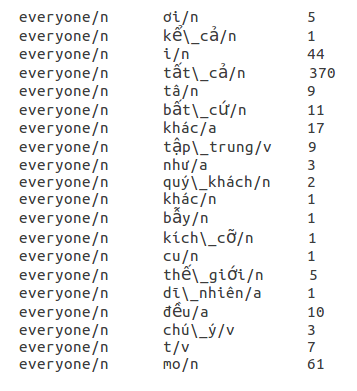
\includegraphics[scale=0.7]{bilingual_sparse_matrix}
	\caption{First 20 lines of the sparse co-occurrence matrix extracted from bilingual corpus}
\end{figure}

Before extraction, because our bilingual corpora are only sentence-aligned, not word-aligned. Hence, fast\_align\cite{dyer2013simple} is used to do the word alignment over 100 iteration.

\begin{minted}{bash}
	log_e likelihood: -7.94319e+07
	log_2 likelihood: -1.14596e+08
	cross entropy: 6.33762
	perplexity: 80.8748
	posterior p0: 0
	posterior al-feat: 0
	size counts: 3680
\end{minted}

\section{Question 10}
For feature weighting scheme, we have these functions to be taken into account:
\begin{itemize}
	\item Vector normalisation which normalises the co-occurrence count into probability distribution (over row or column)
	\item Term Frequency - Inverse Document Frequency (TF-IDF) in case of constructing word-document matrix
	\[tfidf(f,d) = P(w|d)*log\left(\frac{|D|}{|d\in D: w\in d|}\right)\]
	\item Point-wise Mutual Information (PMI), in which t, f are target word, feature word respectively
	\[PMI(t,f)=log\left(\frac{P(t,f)}{P(t)P(f)}\right)\]
	\item Exponential Point-wise Mutual Information (EPMI)
	\[EPMI(t,f)=\frac{P(t,f)}{P(t)P(f)}\]
	\item Positive Point-wise Mutual Information
	\[PPMI(t,f) = max(PMI(t,f), 0)\]
	\item PMI with contextual discounting\cite{pantel2002discovering}, let X be the co-occurrence matrix
	\[cdPMI(t,f)=PMI(t,f)*\frac{X_{tf}}{X_{tf}+1}*\frac{min(\sum_{k=1}^{m}X_{kf},\sum_{k=1}^{n}X_{tk})}{min(\sum_{k=1}^{m}X_{kf},\sum_{k=1}^{n}X_{tk})+1}\]
	\item Positive Local Mutual Information (PLMI)
	\[PLMI(t,f)=PPMI(t,f)*X_{t,f}\]
	\item t-test
	\[\frac{p(t,f)-p(t)p(f)}{\sqrt{p(t)p(f)}}\]
	\item Positive Log Weighting (Plog)
	\[Plog(t,f)=max(0,log(t,f))\]
\end{itemize}

By using raw frequencies without a weighting scheme, we are overrating meaningless words. In TF-IDF perspective, for example, "to be" (after lemmatisation) is a very common word and may occur in the context of many words whereas this does not count much into the target word meaning. In general, word that appears in less context carries more amount of meaning that those appear all over the corpus. TF-IDF helps to prevent these common words to be overrated during our calculation. These other weighting functions do the same thing.

\section{Question 11}
DISSECT comes with 4 weighting schemes: Positive Point-wise Mutual Information (PPMI), Positive Local Mutual Information (PLMI), Exponential Point-wise Mutual Information (EPMI) and Positive Log Weighting (Plog).
This library also provides 4 similarity functions:
\begin{itemize}
	\item Dot product
		\[sim(\vec{u},\vec{v})=\vec{u}.\vec{v}=\sum_iu_iv_i\]
	\item Cosine similarity
		\[sim(\vec{u},\vec{v})=\frac{\vec{u}.\vec{v}}{\sqrt{||\vec{u}||.||\vec{v}||}}\]
	\item Euclidean similarity
		\[sim(\vec{u},\vec{v})=\frac{1}{||\vec{u}-\vec{v}||+1}\]
	\item Lin similarity
		\[sim(\vec{u},\vec{v})=\frac{\sum_{i\in I}(u_i+v_i)}{\sum_iu_i+\sum_iv_i}, I=\{i|u_i>0,v_i>0\}\]
\end{itemize}

In this report, PPMI for weighting is chosen because it is mentioned to be robust by Baroni et al. About the similarity, cosine similarity will do the work, as obviously, direction is more important than distance in this vector space.

\section{Question 12}

% \begin{table}[H]
	\begin{longtable}{ p{7cm} | p{7cm} }
		\textbf{Bilingual} & \textbf{Monolingual}\\
		\hline
		\underline{Top 5 highest frequency} &  \\
		be/v
		\begin{enumerate}
			\item do/v 0.644864852611
			\item have/v 0.53856205691
			\item seem/v 0.501341250193
			\item suppose/v 0.434208274879
			\item appear/v 0.425135594284
		\end{enumerate} & 
		child-n
		\begin{enumerate}
			\item parent-n 0.917077574336
			\item adult-n 0.782701972496
			\item age-v 0.766753507122
			\item mother-n 0.697207331389
			\item care-v 0.672120216415
		\end{enumerate}
		\\
		do/v
		\begin{enumerate}
			\item be/v 0.644864852611
			\item job/n 0.482768427598
			\item miranda/n 0.443403144377
			\item work/v 0.419430517203
			\item happen/v 0.415200117797
		\end{enumerate} &
		company-n
		\begin{enumerate}
			\item firm-n 0.858734913616
			\item sale-n 0.703226771638
			\item share-n 0.692699749645
			\item finance-n 0.679246440312
			\item asset-n 0.673388675912
		\end{enumerate}
		\\
		have/v
		\begin{enumerate}
			\item be/v 0.53856205691
			\item suppose/v 0.463524216234
			\item do/v 0.381634314346
			\item get/v 0.370700718953
			\item guess/v 0.370605030256
		\end{enumerate} &
		government-n
		\begin{enumerate}
			\item reform-n 0.858794556597
			\item opposition-n 0.812902399853
			\item official-n 0.790417186791
			\item citizen-n 0.783790421439
			\item minister-n 0.775312049209
		\end{enumerate}
		\\
		know/v
		\begin{enumerate}
			\item aware/a 0.703021663021
			\item realize/v 0.671213997158
			\item understand/v 0.63907783525
			\item know/n 0.599892302029
			\item knowledge/n 0.55807791604
		\end{enumerate} &
		man-n
		\begin{enumerate}
			\item boy-n 0.808836412112
			\item nothing-n 0.801337325917
			\item suppose-v 0.797160387784
			\item realize-v 0.79553290897
			\item recall-v 0.792342694109
		\end{enumerate}
		\\
		get/v
		\begin{enumerate}
			\item pick/v 0.559988392181
			\item take/v 0.539727747568
			\item catch/v 0.528943028352
			\item grab/v 0.470867631315
			\item bring/v 0.465093376048
		\end{enumerate} &
		interest-n
		\begin{enumerate}
			\item debt-n 0.689492158541
			\item asset-n 0.67486902297
			\item finance-n 0.664138447874
			\item investment-n 0.627399311431
			\item fund-n 0.607052624799
		\end{enumerate}
		\\

		\underline{Top 5 lowest frequency} &  \\
		honor/v
		\begin{enumerate}
			\item honor/n 0.914345975167
			\item respect/n 0.627452925122
			\item proud/a 0.580979180612
			\item pride/n 0.55512987187
			\item pleasure/n 0.518680112168
		\end{enumerate} &
		flinch-v
		\begin{enumerate}
			\item face-n 0.634137640313
			\item turn-v 0.594026517471
			\item moment-n 0.589972389237
			\item throw-v 0.589120941417
			\item hand-n 0.586821526683
		\end{enumerate}
		\\
		cause/n
		\begin{enumerate}
			\item reason/n 0.609092817925
			\item cause/v 0.565175858232
			\item purpose/n 0.516723494415
			\item excuse/n 0.326777208454
			\item regret/v 0.306312326903
		\end{enumerate} &
		digress-v
		\begin{enumerate}
			\item sort-n 0.530770049145
			\item suppose-v 0.506682152561
			\item something-n 0.505936566787
			\item seem-v 0.50282571827
			\item wonder-v 0.500758937318
		\end{enumerate}
		\\
		gut/n
		\begin{enumerate}
			\item courage/n 0.805742297034
			\item brave/v 0.723577063421
			\item dare/v 0.618285158884
			\item capable/a 0.52971806174
			\item ball/n 0.459042016931
		\end{enumerate} &
		ricochet-v
		\begin{enumerate}
			\item shot-n 0.607339659037
			\item ball-n 0.582938290069
			\item hit-v 0.570853829087
			\item strike-v 0.569048093428
			\item throw-v 0.556888195528
		\end{enumerate}
		\\
		friday/n
		\begin{enumerate}
			\item tomorrow/n 0.580693672328
			\item yesterday/n 0.508509729613
			\item sunday/n 0.500100539258
			\item night/n 0.497346989695
			\item tonight/n 0.491611345723
		\end{enumerate} &
		slouch-v
		\begin{enumerate}
			\item sit-v 0.525704745576
			\item back-n 0.500733637246
			\item shoulder-n 0.499656537184
			\item face-n 0.4974346316
			\item notice-v 0.496175792746
		\end{enumerate}
		\\
		criminal/a
		\begin{enumerate}
			\item crime/n 0.887793115624
			\item guilty/a 0.630346289689
			\item robbery/n 0.605219555932
			\item offense/n 0.568078418005
			\item sin/n 0.55002560594
		\end{enumerate} &
		gabble-v
		\begin{enumerate}
			\item talk-v 0.410311235872
			\item wonder-v 0.401321902108
			\item moment-n 0.398461557888
			\item hear-v 0.392450811479
			\item listen-v 0.387854584271
		\end{enumerate}
		\\
		&
		
		\\
	\end{longtable}
% \end{table}

As stated above, running our DSM on bilingual corpora tends to produce higher percentage of synonyms than monolingual corpus. For example, ``know/v" in bilingual corpora goes with ``aware", ``realise", ``understand"... while ``government-n" in monolingual corpus goes with ``reform", ``opposition", ``official", ``citizen"... It is obvious that monolingual corpus propose more topic-related words.

In comparison between high-frequency (HF) and low-frequency (LF) words. Related words for HF words tend to spread broader in meaning than LF words in both corpora. For instance, ``be/v' or ``do/v" in bilingual have a broader range of relatedness because in Vietnamese, these two words can be substituted by a wide range of words depending on context. The same range happens to ``child-n" as well. On the other hand, ``gut/n" in bilingual corpora and ``ricochet-v" in monolingual corpus seem to have more closely related words.

\section{Question 13}
In brief, contextual variability stands for a problem or phenomenon that the meaning we assign for a particular word can be varied depending on the context where that word occurs. Let us take the word ``gut/n" of our bilingual corpora in the list above as an example, its meaning varies from ``intestine", ``belly" to ``courage" or ``determination". However, because of the nature of film subtitles, most of its usage belong to the latter case, in which the related words are listed above.

The difference can be more subtle. For instance, ``I will go to Washington next year" vs. ``Washington declared their stand on the problem". In these sentences, the former ``Washington" is the capital of the United States, while the latter is the U.S. government.

For polysemous word, let us choose the famous ``bank-n".
\begin{enumerate}
	\item bank-n 1.0
	\item cash-n 0.637879447974
	\item finance-n 0.553212523761
	\item debt-n 0.552867349563
	\item money-n 0.549037117541
	\item account-n 0.542203646392
	\item fund-n 0.536145442912
	\item credit-n 0.529048101638
	\item payment-n 0.510477460579
	\item purchase-n 0.507018840735
	\item asset-n 0.505840055635
	\item capital-n 0.497043488885
	\item investment-n 0.491719961594
	\item river-n 0.486462985351
	\item pay-v 0.479063629788
	\item loan-n 0.476691468646
	\item company-n 0.474462371703
	\item invest-v 0.466238846801
	\item firm-n 0.465827345318
	\item exchange-n 0.460229621276
\end{enumerate}

In the list of 19 related words above (except bank-n itself), most of those are about banking and finance (which is one of its sense). Fortunately, the $14^{th}$ word denotes its relation with river (in river bank). This happen because of the dominance of finance-related bank in the corpus, which crawled from newspapers and encyclopedia. The same situation occurs to our ``gut/n" in bilingual corpora. Because of the nature of those corpora (film subtitles), ``gut/n" denotes a kind of human virtue or mental instance instead of a part of human body.

In case of homonyms, let us meet our acquaintances ``present-v" and ``present-n" from question 5.
\begin{longtable}{ p{7cm} | p{7cm} }
	\textbf{present-n} & \textbf{present-v}\\
	\hline
	\begin{enumerate}
		\item gift-n 0.518967672286
		\item living-n 0.488776654395
		\item couple-n 0.484307429417
		\item husband-n 0.44554892667
		\item household-n 0.414977623657
		\item marry-v 0.40744417453
		\item occasion-n 0.404849265528
		\item wedding-n 0.355775154089
		\item past-n 0.333187680494
		\item celebrate-v 0.331177180356
	\end{enumerate}
	&
	\begin{enumerate}
		\item illustrate-v 0.693506315963
		\item presentation-n 0.691251540248
		\item writing-n 0.597135409141
		\item perspective-n 0.577479002089
		\item interpretation-n 0.573946360157
		\item theme-n 0.567569668364
		\item describe-v 0.564004311533
		\item draw-v 0.563206571465
		\item discussion-n 0.552639114303
		\item examine-v 0.54609084858
	\end{enumerate}
	\\
\end{longtable}

In this case, we can see clearly the difference between ``present-n" as ``gift" and ``present-v" as ``to illustrate". This also reconfirms the advantages of using POS information we have discussed in question 5.

\section{Question 14}
According to the principle of compositionality, which is also called Frege's principle, the meaning of a compound is determined by the meanings of its elements and the rules used to combine them. For example, the world ``computer mouse" is constructed from ``computer" and ``mouse", so its meaning should relates to these two words. Moreover, the way ``computer" stands before ``mouse" denotes that the main meaning is ``mouse", and ``computer" specifies this kind of ``mouse", keeps it separated from others.

To be adapted to compositionality, there are several ways. One simple solution is to treat these compound word as a single units (which is somehow already solve in Vietnamese tokenisation). The other way is to perceive compositionality as a function. This approach is implemented by a various sets of functions: additive, full additive, weighted additive, multiplicative, lexical, full lexical, dilation...

\section{Question 15}
DISSECT provides us with full and weighted additive, multiplicative, dilation and lexical function. Hence, we choose lexical function to perform our tasks. This justification is based on a work of compositional DSM evaluation from Dinu et al.\cite{dinu2013general}. In their explanation, lexical function works pretty well because it considers linguistic relations between words (verb-object, verb-subject or modification relations...).

To re-run the experiment, please use: \mint{bash}{bash run_comp.sh}

Our outputs from the command above are:
\begin{longtable}{ p{2cm} | p{5cm} | p{5cm} }
	& \textbf{Argument space} & \textbf{Observed phrase space}\\
	\hline
	ball-n\newline ricochet-v &
	\begin{enumerate}
		\item shot-n 0.60090820919
        \item ball-n 0.555601914406
        \item ricochet-v 0.549424934767
        \item hit-v 0.512803151047
        \item yard-n 0.486374884256
        \item flick-v 0.483794412282
        \item fire-v 0.463375541489
        \item shoot-v 0.45805234635
        \item drop-v 0.450721566791
        \item strike-v 0.437304242189
	\end{enumerate}
	&
	\begin{enumerate}
		\item ball-n\_ricochet-v 1.0
		\item shot-n\_ricochet-v 0.943434619602
		\item ball-n\_rebound-v 0.469537442791
		\item share-n\_ricochet-v 0.417981793027
		\item hand-n\_kick-v 0.390882784654
		\item optimism-n\_ricochet-v 0.374202443085
		\item head-n\_shudder-v 0.323837743214
		\item rifle-n\_recoil-v 0.308846129507
		\item screen-n\_flick-v 0.307706335726
		\item eye-n\_flare-v 0.303568463715
	\end{enumerate}
	\\
	vein-n\newline pulse-v &
	\begin{enumerate}
		\item entrance-n 0.224424352834
		\item tower-n 0.200311482731
		\item paint-v 0.199348815366
		\item hill-n 0.193616827569
		\item road-n 0.193117821902
		\item wall-n 0.188580909673
		\item floor-n 0.186548341616
		\item west-n 0.182714679164
		\item stone-n 0.180126459453
		\item north-n 0.1797992173
	\end{enumerate}
	&
	\begin{enumerate}
        \item vein-n\_pulse-v 1.0
        \item voice-n\_pulse-v 0.318874524154
        \item export-n\_thunder-v 0.199271833659
        \item face-n\_beam-v 0.198910407124
        \item cigar-n\_glow-v 0.169324448505
        \item head-n\_stoop-v 0.168784963436
        \item child-n\_roam-v 0.162331076115
        \item cigar-n\_burn-v 0.155946374982
        \item fountain-n\_erupt-v 0.139816664857
        \item fire-n\_beam-v 0.139524551862
	\end{enumerate}
	\\
	\hline
\end{longtable}

It is clear that in the argument space, the neighbours are both related to one of the two words made up our compound word. While in the observed phrase space, the neighbours are those similar in both meanings of each constituent and meaning constructed by combining all of its constituents.

\section{Question 16}
We can not create a compositional model for our bilingual corpora as the way we did in question 15. The compositional models in DISSECT require observed phrase corpus to be extracted with linguistic relations (subject-verb in case of DISSECT data). Whereas, the relation of pairs in bilingual data is alignment between different language corpora, not within the corpus itself.

\section{Question 17}
In plain, prototype theory states that some members of a category are more central than others. Hence, it creates a graded categorisation for that category by ``distance" to its central one, or prototype. By that theory, meaning of concept/object in lexical semantics can be expressed not by some well-defined features but its similarity in some of its features.

For example, if we defines the word ``bird" for animal with ``wing" and ``ability to fly", ``eagle" is clearly a hyponym of ``bird", ``chicken" is to be considered, while ``ostrich" or ``penguin" will be out due to their lack of needed feature(s). However, in prototype theory, ``eagle", by all ``bird" requirements, can be chosen as ``prototype", and ``chicken" or ``ostrich" and ``penguin" can be in the graded categorisation system (somehow farther than ``pigeon") due to its similarity to the prototype. Consequently, the hyponymous relations in these cases are also constructed via this graded categorisation.

\section{Question 18}
Let compute the neighbours for ``knife/n" in our bilingual corpora:
\begin{enumerate}
	\item knife/n 1.0
	\item blade/n 0.846837062401
	\item sword/n 0.757256934822
	\item throat/n 0.46765543662
	\item cut/v 0.421440081426
	\item cut/n 0.411966698543
	\item stick/v 0.398805264072
	\item wood/n 0.392601946913
	\item stick/n 0.383138407667
	\item tree/n 0.359358089655
	\item tongue/n 0.349288518585
	\item bite/v 0.339242334869
	\item finger/n 0.312515569684
	\item back/n 0.308099197181
	\item wound/n 0.298108472021
	\item side/n 0.271557471912
	\item teeth/n 0.269856045383
	\item skill/n 0.265075315182
	\item arrow/n 0.255360859053
	\item iron/n 0.252328951782
\end{enumerate}

It is obvious that ``blade", ``sword" are closer to ``knife" in the category of ``personal hand-held ancient close-combat weapons". Those which are in outer level of this category can also be found as ``stick" (not so harmful), teeth (not hand-held), arrow (not for close combat) with less score. Therefore, DSM seems to cater for typicality effect.

\bibliography{report}{}
\bibliographystyle{apalike}

\end{document}          
